\documentclass[conference]{IEEEtran}

% ---------- Packages ----------
\usepackage{newtxtext,newtxmath}
\usepackage{amsmath}
\usepackage{siunitx}
\usepackage{graphicx,xcolor}
\usepackage{booktabs}
\usepackage{placeins}
\usepackage[hidelinks]{hyperref}
\usepackage{enumitem} % ← リスト圧縮

\usepackage{tikz}
\usetikzlibrary{calc,positioning,fit,arrows.meta,shapes.geometric,shapes.misc,topaths}

% ---------- Compact spacing (IEEEtran安全範囲で軽めに) ----------
\setlength{\textfloatsep}{6pt plus 1pt minus 2pt}
\setlength{\floatsep}{6pt plus 1pt minus 2pt}
\setlength{\intextsep}{6pt plus 1pt minus 2pt}
\setlength{\abovecaptionskip}{2pt plus 1pt minus 1pt}
\setlength{\belowcaptionskip}{0pt}
\setlist[itemize]{noitemsep, topsep=1pt, leftmargin=*, parsep=0pt, partopsep=0pt}

% ---------- TikZ styles ----------
\tikzset{
  line/.style = {-{Latex}, line width=0.5pt},
  box/.style  = {draw, rounded corners, align=center, inner sep=3pt},
  smallbox/.style = {box, minimum width=28mm, minimum height=7mm},
  midbox/.style   = {box, minimum width=36mm, minimum height=8mm},
  bigbox/.style   = {box, minimum width=68mm, minimum height=9mm},
  flowstep/.style = {box, minimum width=36mm, minimum height=7mm, fill=black!5},
}

% ---------- Title ----------
\title{AITL on Space: A Robust Three-Layer Architecture\\
with a Tri-NVM Hierarchy (SRAM / MRAM / FRAM)\\
for Long-Duration Spacecraft Autonomy}

\author{
\IEEEauthorblockN{Shinichi Samizo}
\IEEEauthorblockA{Independent Semiconductor Researcher\\
Former Engineer at Seiko Epson Corporation\\
Email: shin3t72@gmail.com\quad GitHub: \url{https://github.com/Samizo-AITL}}
}

\begin{document}
\maketitle

\begin{abstract}
We propose \emph{AITL on Space}, a robust three-layer control architecture (Robust Core, FSM Supervisor, AI Adaptor) integrated with a tri-NVM hierarchy (SRAM/MRAM/FRAM) and mapped to a 22\,nm FD\!SOI SoC. The contribution is a complete end-to-end design flow from mission-level specification to ASIC: requirements are formalized as JSON via \textit{EduController}, synthesized by the \textit{AITL-H} module, validated in FPGA HIL with fault injection, stress-tested through \textit{SystemDK FEM} (thermal/radiation/packaging), and finally implemented as ASIC. This methodology enables resilient autonomy for long-duration spacecraft missions.
\end{abstract}

\section{Introduction}
Deep-space missions require ultra-robust control under total ionizing dose (TID), single event effects (SEE), and thermal cycling. Conventional PID\,+\,Flash architectures face lifetime limits due to charge-trap drift and endurance. We present \textit{AITL on Space}: a resilient three-layer architecture with a tri-NVM hierarchy and a reproducible design flow from specification to ASIC.

\section{Specification and Design Flow}
The process begins with \textbf{Mission Specification}. Requirements such as pointing accuracy, power stability, and thermal tolerance are captured in \textbf{EduController}, a model-based tool that exports plant matrices and weighting functions as JSON (portable across simulators). The JSON is consumed by \textbf{AITL-H}, which synthesizes an $H_\infty$ output-feedback controller $K$ with mixed-sensitivity weighting and generates a fixed-point implementation for RTL/FPGA/ASIC. The design then undergoes:
\begin{itemize}
  \item \textbf{FPGA HIL}: hardware-in-the-loop validation with SEU and outage injection; metrics include safe-mode entry $<\SI{1}{s}$, recovery rate $\ge\SI{99}{\percent}$, and ECC scrubbing efficiency.
  \item \textbf{SystemDK FEM}: FE co-simulation of thermal cycles, radiation effects, and packaging stress, closing the verification loop before silicon.
  \item \textbf{ASIC Mapping}: implementation on GlobalFoundries 22FDX FD\!SOI hardened for long-duration missions.
\end{itemize}

\noindent\textit{Toolchain at a Glance.}
\textbf{EduController}=\;spec$\to$JSON exporter (plant $A,B,C,D$, $E$, noise; weights $W_1,W_2,W_3$). 
\textbf{AITL-H}=\;$H_\infty$ synthesizer (Riccati/LMIs)$\to$ fixed-point $K$(範囲/スケーリング付き). 
\textbf{SystemDK FEM}=\;thermal/radiation/packaging derating \& memory scrubbing validation.

\section{System Architecture}
AITL consists of three layers:
\begin{itemize}
  \item \textbf{Robust Core}: $H_\infty$/MPC/SMC controllers for stability.
  \item \textbf{FSM Supervisor}: Safe/Nominal/Recovery with FDI/FDII.
  \item \textbf{AI Adaptor}: long-term re-identification and drift compensation.
\end{itemize}
A tri-NVM hierarchy ensures persistence: SRAM for execution, MRAM for logs/code with ECC scrubbing and dual slots, and FRAM for safe boot and FSM states. Target SoC is 22\,nm FD\!SOI.

\section{Mathematical Model and \texorpdfstring{$H_\infty$}{H-infinity} Design}
We consider an 11D discrete-time plant coupling attitude (6), power bus (2), and thermal nodes (3):
\begin{align}
  x_{k+1} &= A x_k + B u_k + E w_k, \label{eq:ss1}\\
  y_k &= C x_k + D u_k + v_k. \label{eq:ss2}
\end{align}
$w_k$ and $v_k$ are disturbance and noise. The model extends to 20D by adding translational axes and bias states. Weights $(W_1,W_2,W_3)$ shape sensitivity, control effort, and complementary sensitivity. EduController outputs JSON; AITL-H synthesizes $K$ with robustness margins and exports a fixed-point realization for RTL/FPGA/ASIC.

\section{Verification Pipeline}
FPGA HIL injects SEU bursts and sensor outages. Metrics include safe-mode entry time ($<\SI{1}{s}$), recovery rate ($\ge\SI{99}{\percent}$), and ECC scrubbing efficiency. SystemDK FEM validates thermal and radiation stress, ensuring packaging reliability before ASIC tape-out.

\section{Conclusion}
AITL on Space combines robust control, supervisory safety, AI re-identification, and hardened memory. The proposed end-to-end flow—from mission specification to ASIC—provides a reproducible methodology for resilient autonomy in long-duration space missions.

% ---------- References ----------
\begin{thebibliography}{99}
\bibitem{doyle}
J.\,C.~Doyle, B.\,A.~Francis, and A.\,R.~Tannenbaum,
\emph{Feedback Control Theory}. Macmillan, 1992.

\bibitem{colinge}
J.-P.~Colinge, \emph{Silicon-on-Insulator Technology: Materials to VLSI}, 3rd~ed. Springer, 2004.

\bibitem{wolf}
W.~Wolf, \emph{FPGA-Based System Design}. Prentice Hall, 2004.

\bibitem{rabaey}
J.~M.~Rabaey, A.~Chandrakasan, and B.~Nikoli\'c,
\emph{Digital Integrated Circuits: A Design Perspective}, 2nd~ed. Prentice Hall, 2003.
\end{thebibliography}

% ---------- Biography ----------
\section*{Author Biography}
Shinichi Samizo received the M.S.\ degree in Electrical and Electronic Engineering from Shinshu University, Japan. He worked at Seiko Epson Corporation as an engineer in semiconductor memory and mixed-signal device development, and contributed to inkjet MEMS actuators and PrecisionCore printhead technology. He is currently an independent semiconductor researcher focusing on process/device education, memory architecture, and AI system integration. Contact: \texttt{shin3t72@gmail.com}.

% ---------- All Figures at the End (packed to fit 2 pages) ----------
\section*{Figures}

% ---- Fig.1: Flow (縮小して列幅に合わせる) ----
\begin{figure}[!t]
\centering
\resizebox{\columnwidth}{!}{%
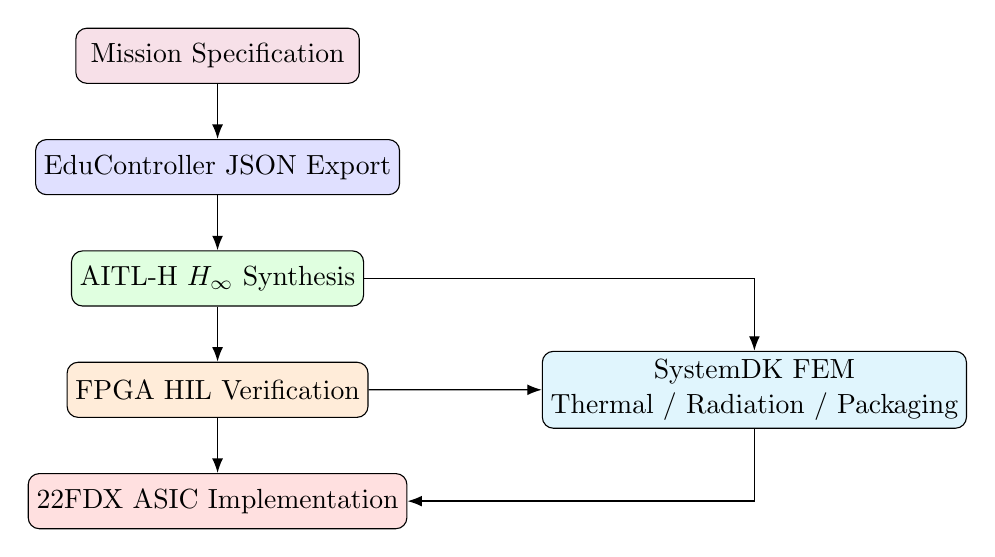
\begin{tikzpicture}[node distance=7mm, scale=0.95]
  \node[flowstep, fill=purple!12] (spec) {Mission Specification};
  \node[flowstep, fill=blue!12, below=of spec] (json) {EduController JSON Export};
  \node[flowstep, fill=green!12, below=of json] (hinf) {AITL-H $H_\infty$ Synthesis};
  \node[flowstep, fill=orange!15, below=of hinf] (hil) {FPGA HIL Verification};
  \node[flowstep, fill=red!12, below=of hil] (asic) {22FDX ASIC Implementation};
  \node[flowstep, fill=cyan!12, right=22mm of hil] (fem) {\shortstack{SystemDK FEM\\Thermal / Radiation / Packaging}};
  \draw[line] (spec) -- (json);
  \draw[line] (json) -- (hinf);
  \draw[line] (hinf) -- (hil);
  \draw[line] (hil) -- (asic);
  \draw[line] (hinf.east) -| (fem.north);
  \draw[line] (hil.east)  -- (fem.west);
  \draw[line] (fem.south) |- (asic.east);
\end{tikzpicture}}
\caption{End-to-end design flow: Mission Spec $\rightarrow$ JSON $\rightarrow$ AITL-H $\rightarrow$ FPGA HIL $\rightarrow$ FEM $\rightarrow$ ASIC.}
\label{fig:flow}
\vspace{-2mm}
\end{figure}

% ---- Fig.2: Architecture + Loop を横並びで1図に統合 ----
\begin{figure}[!t]
\centering
\begin{minipage}[t]{0.55\columnwidth}
\centering
\resizebox{\linewidth}{!}{%
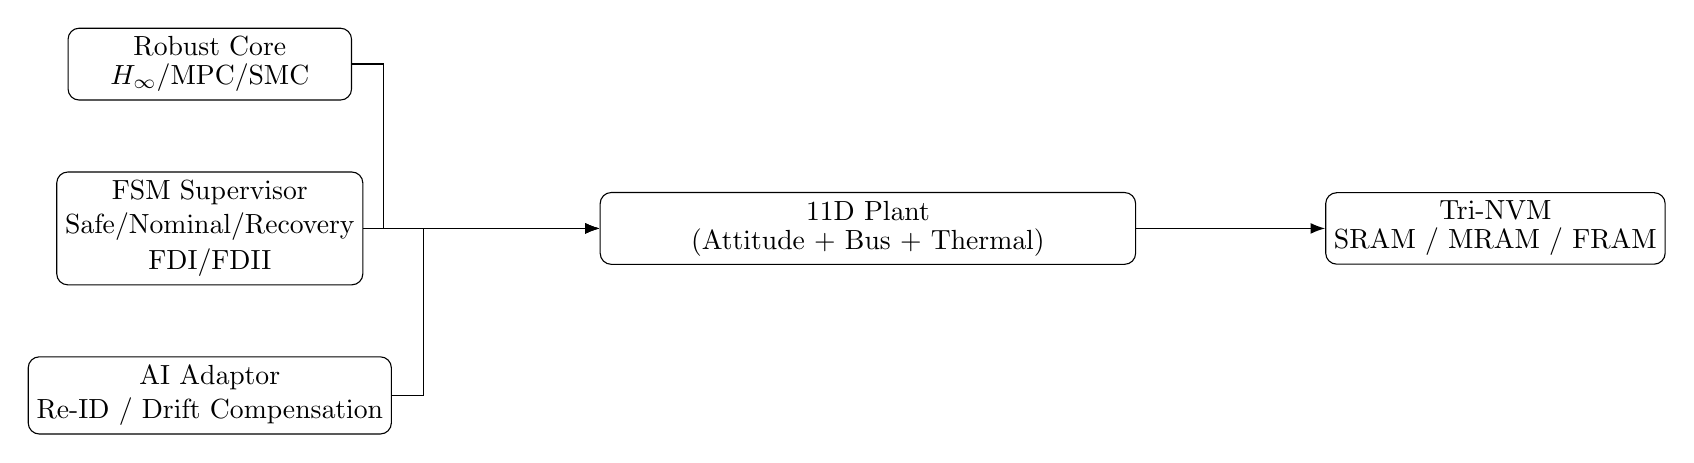
\begin{tikzpicture}[node distance=7mm]
  \node[midbox] (core) {\shortstack{Robust Core\\$H_\infty$/MPC/SMC}};
  \node[midbox, below=9mm of core] (fsm) {\shortstack{FSM Supervisor\\Safe/Nominal/Recovery\\FDI/FDII}};
  \node[midbox, below=9mm of fsm] (ai) {\shortstack{AI Adaptor\\Re-ID / Drift Compensation}};
  \node[bigbox, right=30mm of fsm] (plant) {\shortstack{11D Plant\\(Attitude + Bus + Thermal)}};
  \node[midbox, right=24mm of plant] (nvm) {\shortstack{Tri-NVM\\SRAM / MRAM / FRAM}};
  \draw[line] (core.east) -| ($(core.east)+(4mm,0)$) |- (plant.west);
  \draw[line] (fsm.east) -- (plant.west);
  \draw[line] (ai.east)  -| ($(ai.east)+(4mm,0)$) |- (plant.west);
  \draw[line] (plant.east) -- (nvm.west);
\end{tikzpicture}}
\end{minipage}\hfill
\begin{minipage}[t]{0.4\columnwidth}
\centering
\resizebox{\linewidth}{!}{%
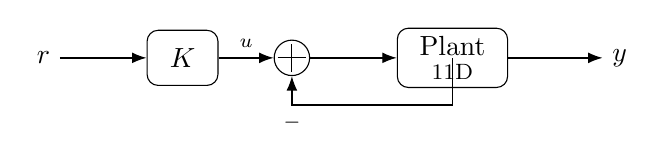
\begin{tikzpicture}[node distance=7mm]
  \node[smallbox, minimum width=9mm] (K) {$K$};
  \node[circle, draw, minimum size=4.5mm, right=7mm of K] (sum) {};
  \draw (sum) +(-1.8mm,0) -- +(1.8mm,0);
  \draw (sum) +(0,-1.8mm) -- +(0,1.8mm);
  \node[smallbox, right=11mm of sum, minimum width=14mm] (P) {\shortstack{Plant\\\footnotesize 11D}};
  \node[right=12mm of P] (y) {$y$};
  \node[left=11mm of K] (r) {$r$};
  \draw[line] (r) -- (K);
  \draw[line] (K) -- node[above]{\scriptsize $u$} (sum);
  \draw[line] (sum) -- (P);
  \draw[line] (P) -- (y);
  \draw[line] ($(P.north)!0.5!(P.south)$) |- ++(0,-6mm) -| node[below]{\scriptsize $-$} (sum.south);
\end{tikzpicture}}
\end{minipage}
\caption{(Left) AITL architecture with tri-NVM hierarchy (orthogonal wiring). (Right) Closed-loop for $H_\infty$ mixed-sensitivity on the 11D plant.}
\label{fig:archloop}
\vspace{-2mm}
\end{figure}

% ページ最終段の2段長合わせ(必要に応じて行番号を調整)
\IEEEtriggeratref{3}

\end{document}
